\documentclass[journal,12pt,twocolumn]{IEEEtran}

\usepackage{setspace}
\usepackage{gensymb}

\singlespacing


\usepackage[cmex10]{amsmath}

\usepackage{amsthm}

\usepackage{mathrsfs}
\usepackage{txfonts}
\usepackage{stfloats}
\usepackage{bm}
\usepackage{cite}
\usepackage{cases}
\usepackage{subfig}

\usepackage{longtable}
\usepackage{multirow}

\usepackage{enumitem}
\usepackage{mathtools}
%\usepackage{steinmetz}
\usepackage{tikz}
\usepackage{circuitikz}
\usepackage{verbatim}
%\usepackage{tfrupee}
\usepackage[breaklinks=true]{hyperref}

\usepackage{tkz-euclide}

\usetikzlibrary{calc,math}
\usepackage{listings}
    \usepackage{color}                                            %%
    \usepackage{array}                                            %%
    \usepackage{longtable}                                        %%
    \usepackage{calc}                                             %%
    \usepackage{multirow}                                         %%
    \usepackage{hhline}                                           %%
    \usepackage{ifthen}                                           %%
    \usepackage{lscape}     
\usepackage{multicol}
\usepackage{chngcntr}

\DeclareMathOperator*{\Res}{Res}

\renewcommand\thesection{\arabic{section}}
\renewcommand\thesubsection{\thesection.\arabic{subsection}}
\renewcommand\thesubsubsection{\thesubsection.\arabic{subsubsection}}

\renewcommand\thesectiondis{\arabic{section}}
\renewcommand\thesubsectiondis{\thesectiondis.\arabic{subsection}}
\renewcommand\thesubsubsectiondis{\thesubsectiondis.\arabic{subsubsection}}


\hyphenation{op-tical net-works semi-conduc-tor}
\def\inputGnumericTable{}                                 %%

\lstset{
%language=C,
frame=single, 
breaklines=true,
columns=fullflexible
}
\begin{document}


\newtheorem{theorem}{Theorem}[section]
\newtheorem{problem}{Problem}
\newtheorem{proposition}{Proposition}[section]
\newtheorem{lemma}{Lemma}[section]
\newtheorem{corollary}[theorem]{Corollary}
\newtheorem{example}{Example}[section]
\newtheorem{definition}[problem]{Definition}

\newcommand{\BEQA}{\begin{eqnarray}}
\newcommand{\EEQA}{\end{eqnarray}}
\newcommand{\define}{\stackrel{\triangle}{=}}
\bibliographystyle{IEEEtran}
\providecommand{\mbf}{\mathbf}
\providecommand{\pr}[1]{\ensuremath{\Pr\left(#1\right)}}
\providecommand{\qfunc}[1]{\ensuremath{Q\left(#1\right)}}
\providecommand{\sbrak}[1]{\ensuremath{{}\left[#1\right]}}
\providecommand{\lsbrak}[1]{\ensuremath{{}\left[#1\right.}}
\providecommand{\rsbrak}[1]{\ensuremath{{}\left.#1\right]}}
\providecommand{\brak}[1]{\ensuremath{\left(#1\right)}}
\providecommand{\lbrak}[1]{\ensuremath{\left(#1\right.}}
\providecommand{\rbrak}[1]{\ensuremath{\left.#1\right)}}
\providecommand{\cbrak}[1]{\ensuremath{\left\{#1\right\}}}
\providecommand{\lcbrak}[1]{\ensuremath{\left\{#1\right.}}
\providecommand{\rcbrak}[1]{\ensuremath{\left.#1\right\}}}
\theoremstyle{remark}
\newtheorem{rem}{Remark}
\newcommand{\sgn}{\mathop{\mathrm{sgn}}}
\providecommand{\abs}[1]{\left\vert#1\right\vert}
\providecommand{\res}[1]{\Res\displaylimits_{#1}} 
\providecommand{\norm}[1]{\left\lVert#1\right\rVert}
%\providecommand{\norm}[1]{\lVert#1\rVert}
\providecommand{\mtx}[1]{\mathbf{#1}}
\providecommand{\mean}[1]{E\left[ #1 \right]}
\providecommand{\fourier}{\overset{\mathcal{F}}{ \rightleftharpoons}}
%\providecommand{\hilbert}{\overset{\mathcal{H}}{ \rightleftharpoons}}
\providecommand{\system}{\overset{\mathcal{H}}{ \longleftrightarrow}}
	%\newcommand{\solution}[2]{\textbf{Solution:}{#1}}
\newcommand{\solution}{\noindent \textbf{Solution: }}
\newcommand{\cosec}{\,\text{cosec}\,}
\providecommand{\dec}[2]{\ensuremath{\overset{#1}{\underset{#2}{\gtrless}}}}
\newcommand{\myvec}[1]{\ensuremath{\begin{pmatrix}#1\end{pmatrix}}}
\newcommand{\mydet}[1]{\ensuremath{\begin{vmatrix}#1\end{vmatrix}}}
\numberwithin{equation}{subsection}
\makeatletter
\@addtoreset{figure}{problem}
\makeatother
\let\StandardTheFigure\thefigure
\let\vec\mathbf
\renewcommand{\thefigure}{\theproblem}
\def\putbox#1#2#3{\makebox[0in][l]{\makebox[#1][l]{}\raisebox{\baselineskip}[0in][0in]{\raisebox{#2}[0in][0in]{#3}}}}
     \def\rightbox#1{\makebox[0in][r]{#1}}
     \def\centbox#1{\makebox[0in]{#1}}
     \def\topbox#1{\raisebox{-\baselineskip}[0in][0in]{#1}}
     \def\midbox#1{\raisebox{-0.5\baselineskip}[0in][0in]{#1}}
\vspace{3cm}
\title{EE5609 Assignment 6}
\author{SHANTANU YADAV, EE20MTECH12001 }
\maketitle
\newpage
\bigskip
\renewcommand{\thefigure}{\theenumi}
\renewcommand{\thetable}{\theenumi}

The python solution code is available at
\begin{lstlisting}
https://github.com/Shantanu2508/Matrix_Theory/blob/master/Assignment_6/assignment6.py
\end{lstlisting}

\section{Problem}
What conic does the following equation represent? Find its equation and centre.
\begin{align*}
	3x^2 - 8xy - 3y^2 + 10x - 13y + 8 =0 
\end{align*}

\section{Solution}
The general equation of second degree can be expressed as
\begin{align}
	\vec{x}^{T}\vec{Vx} + 2\vec{u}^{T}\vec{x} + f=0   \label{stdsecdeg}
\end{align}
where
\begin{align}
        \vec{V}=\vec{V}^T=\myvec{a & b \\ b & c}   \label{V}  \\
        \vec{u}^T=\myvec{d &  e}            \label{u}
\end{align}
From (\ref{V}) and (\ref{u})
\begin{align}
	\vec{V}=\vec{V}^T &= \myvec{3 & -4 \\ -4 & -3} \\
	\vec{u} &= \myvec{5 \\ -\frac{13}{2}}
\end{align}
\begin{align}
	\mydet{\vec{V}}=\mydet{3 & -4 \\ -4 & 3} =-25 \\
	\implies \mydet{\vec{V}} < 0       \label{detless0}
\end{align}
Since $ \vec{V} = \vec{V}^T $, there exists an orthogonal matrix $\vec{P}$ such that
\begin{align}
	\vec{P}\vec{V}\vec{P}^T = \vec{D} = diag\myvec{\lambda_1 & \lambda_2}
\end{align}
or equivalently 
\begin{align}
	\vec{V} = \vec{P}\vec{D}\vec{P}^T
\end{align}
Eigen vectors of real symmetric matrix $\vec{V}$ are orthogonal. The characteristic equation of $\vec{V}$ is obtained by evaluating the determinant
\begin{align}
	\mydet{\lambda\vec{I}-\vec{V}} = \mydet{\lambda-3 & 4 \\ 4 & \lambda + 3} = 0 \\
	\implies \quad \lambda^2-25=0 \\
	\implies \quad \lambda_1=-5,\lambda_2=5   \label{lambdavals}
\end{align}
From (\ref{detless0}) and (\ref{lambdavals}) the equation represents a hyperbola.
The eigen vector $\vec{p}$ is defined as
\begin{align}
	\vec{V}\vec{p}=\lambda\vec{p} \\
	\implies (\lambda\vec{I} - \vec{V})\vec{p}=0
\end{align}
For $\lambda_1 = -5$ :
\begin{align}
	(\lambda_1\vec{I}-\vec{V})=\myvec{-8 & 4 \\ 4 & -2} 
	\xleftrightarrow[R_2 \leftarrow \frac{R_2}{2}]{R_1 \leftarrow -\frac{R_1}{4}}
	\myvec{2 & -1 \\ 2 & -1} \\
	\xleftrightarrow[]{R_2 \leftarrow R_2 - R_1}
	\myvec{2 & -1 \\ 0 & 0} \\
	\implies \vec{p_1}=\frac{1}{\sqrt{5}}\myvec{2 \\ 1}
\end{align}
Similarly, the eigenvector corresponding to $\lambda_2$ can be obtained as
\begin{align}
	\vec{p_2}=\frac{1}{\sqrt{5}}\myvec{-1\\2}
\end{align}
The orthogonal eigen-vector matrix
\begin{align}
	\vec{P}=\myvec{\vec{p_1} & \vec{p_2}}
	=\frac{1}{\sqrt{5}}\myvec{2 & -1 \\ 1 & 2} \\
	\vec{D}=\myvec{-5 & 0 \\ 0 & 5}
\end{align}
Let $\vec{x}=\vec{P}\vec{y} + \vec{c} $ with $\vec{c}=-\vec{V}^{-1}\vec{u}$. Substituting in (\ref{stdsecdeg})
\begin{align}
	\vec{y}^T\vec{D}\vec{y}=\vec{u}^T\vec{V}^{-1}\vec{u}-f 
\end{align}
with centre
\begin{align}
	\vec{c}=-\vec{V^{-1}u}=\myvec{-\frac{41}{25} \\ \frac{1}{50}} 
\end{align}
and minor and major axes parameters as
\begin{align}
	\sqrt{\frac{\lambda_1}{f-\vec{u^{T}V^{-1}u}}} = \sqrt{\frac{500}{33}}, \
	\sqrt{\frac{\lambda_2}{\vec{u^{T}V^{-1}u}-f}} = \sqrt{\frac{500}{33}}
\end{align}
The equation of hyperbola is
\begin{align}
	\frac{y_2^2}{\frac{33}{500}}-\frac{y_1^2}{\frac{33}{500}}=1
\end{align}
\begin{figure}[!h]
	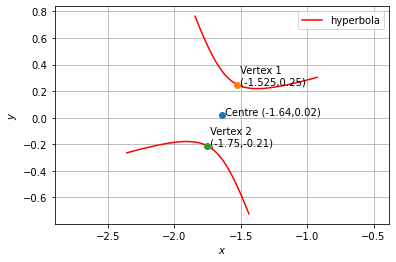
\includegraphics[width=\columnwidth]{hyper.png}
	\caption{} \label{linefig1}
\end{figure}
\end{document}
